\documentclass[11pt]{beamer}
\usetheme{Warsaw}
\usepackage[utf8]{inputenc}
\usepackage[german]{babel}
\usepackage[T1]{fontenc}
\usepackage{amsmath}
\usepackage{amsfonts}
\usepackage{amssymb}
\usepackage{graphicx}
\usepackage{caption}
\usepackage{subcaption}
\usepackage{float}

\author{Stefan Zaufl, Christian Brändle, Dominik Schörkhuber}
\title{3D Vision UE}
%\setbeamercovered{transparent} 
%\setbeamertemplate{navigation symbols}{} 
%\logo{} 
%\institute{} 
%\date{} 
%\subject{} 

\begin{document}

\begin{frame}
\titlepage
\end{frame}

%\begin{frame}
%\tableofcontents
%\end{frame}

\begin{frame}{Mann-Modell}
	\begin{columns}
	\column{.3\textwidth}
		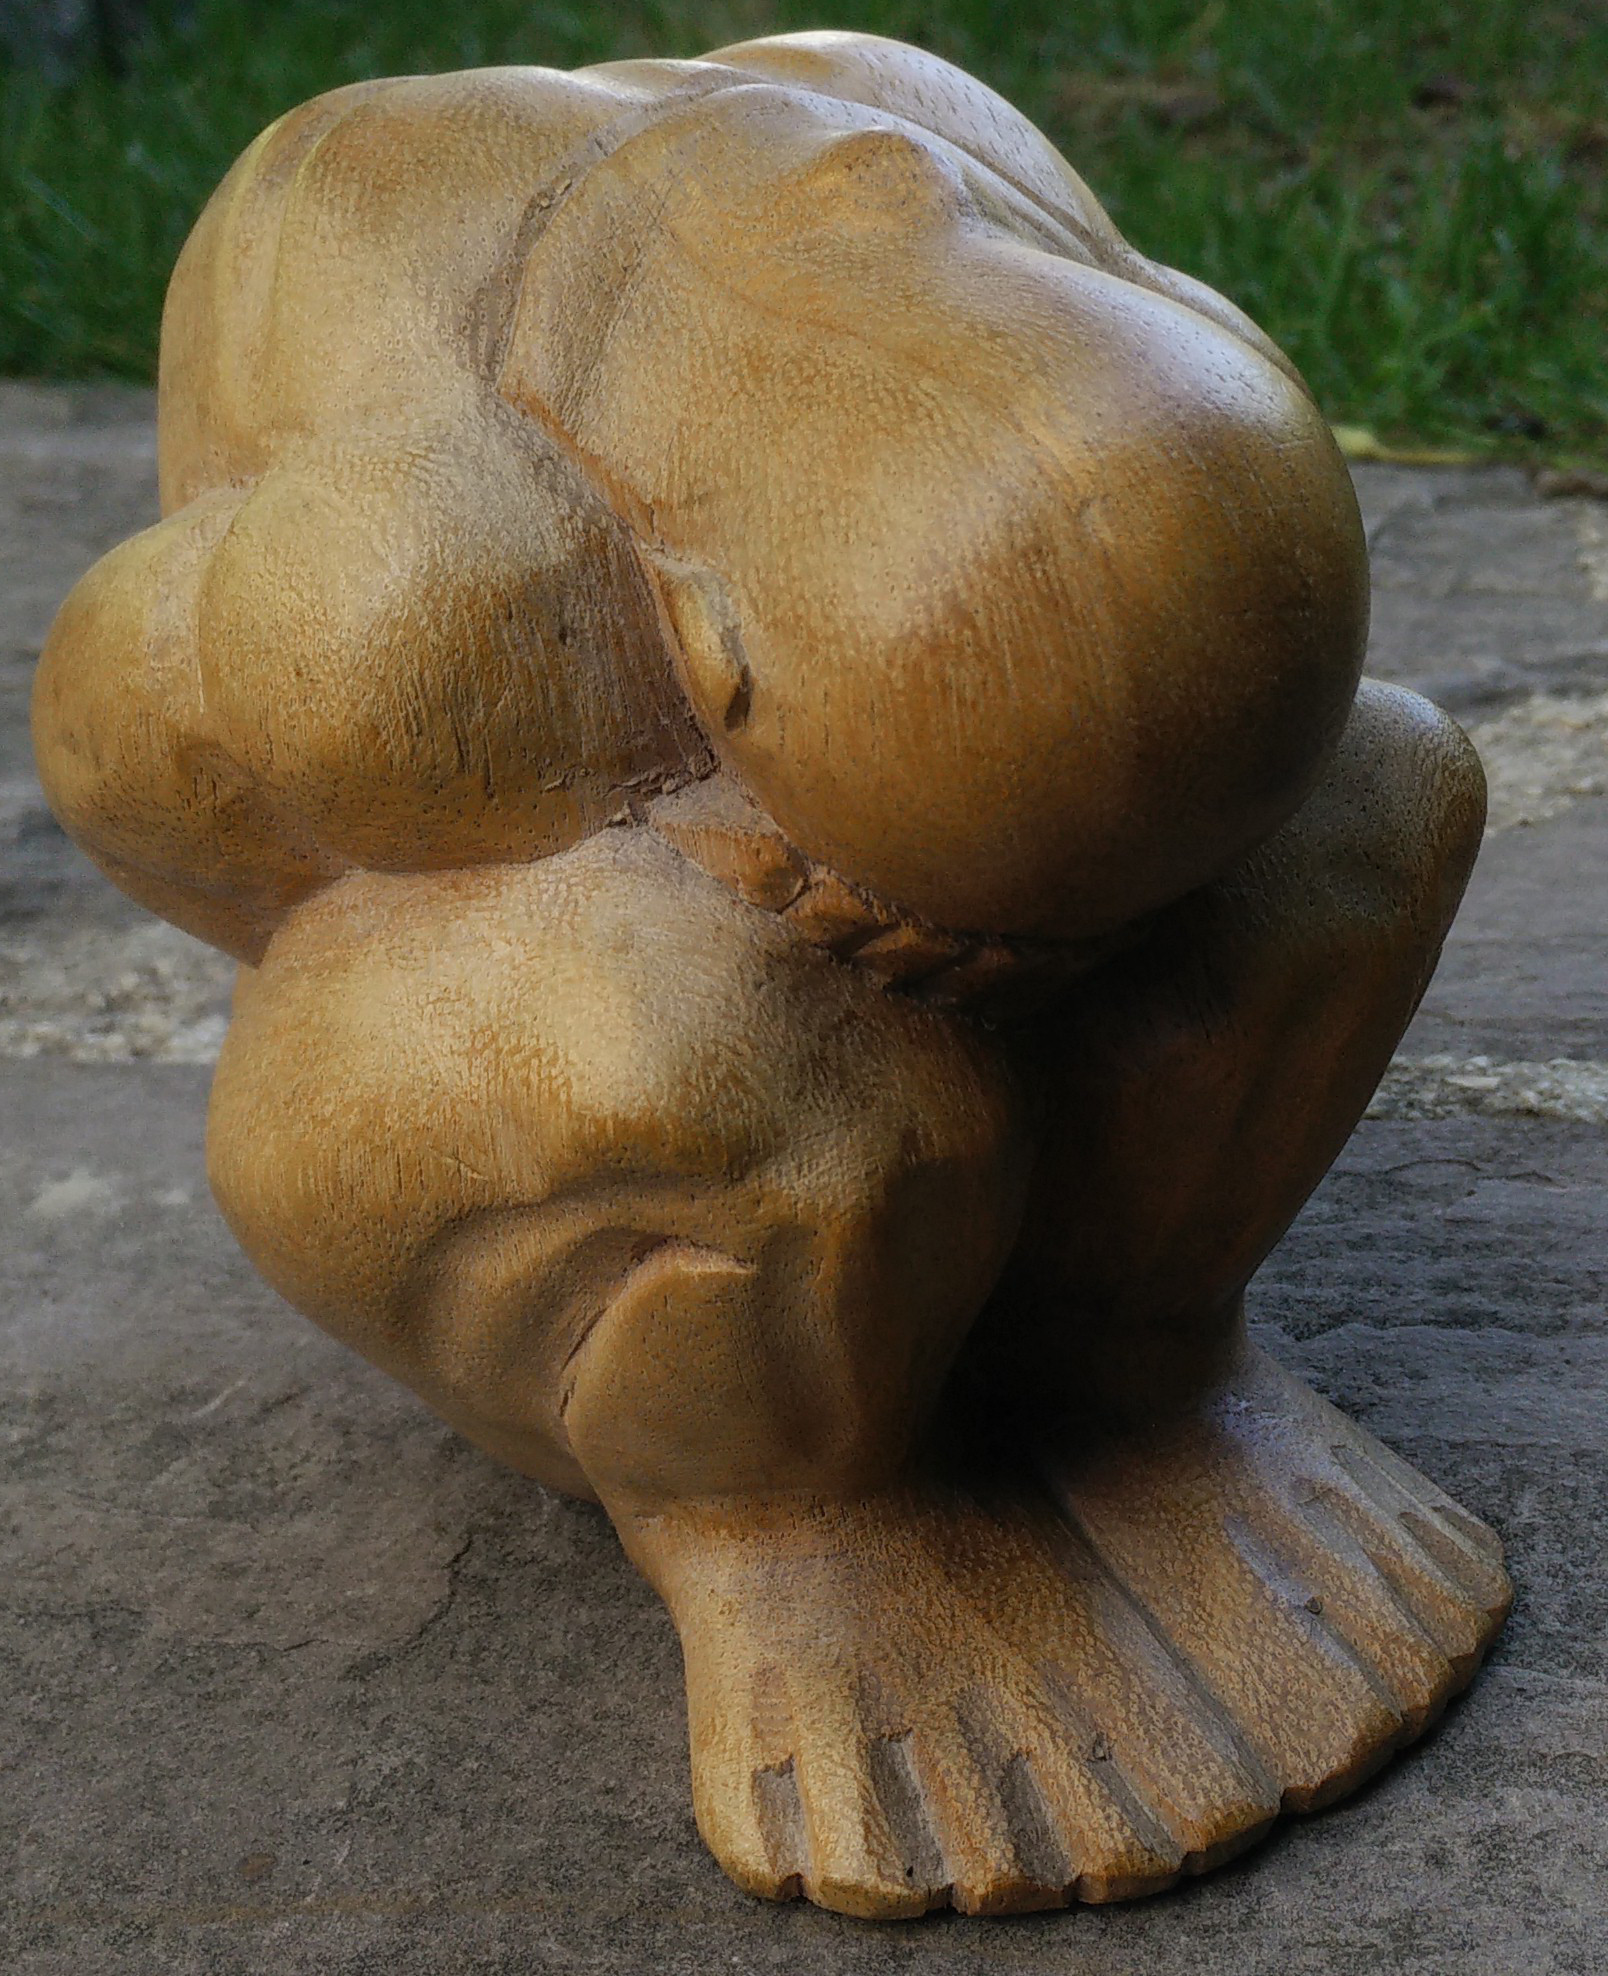
\includegraphics[width=3.5cm]{images/Mann_Original.jpg}
	\column{.7\textwidth}
		\begin{itemize}
		\item Kleine Figur aus Holz
		\item Hat durch die Maserung eine gute Textur
		\item Form annähernd eine Kugel
		\item Problemstellen: konkave Regionen (z.B. bei den Armen) 
		\end{itemize}
	\end{columns}
\end{frame}

\begin{frame}{Mann-Modell: Scan}
	\begin{figure}
		\begin{subfigure}{0.4\textwidth}
			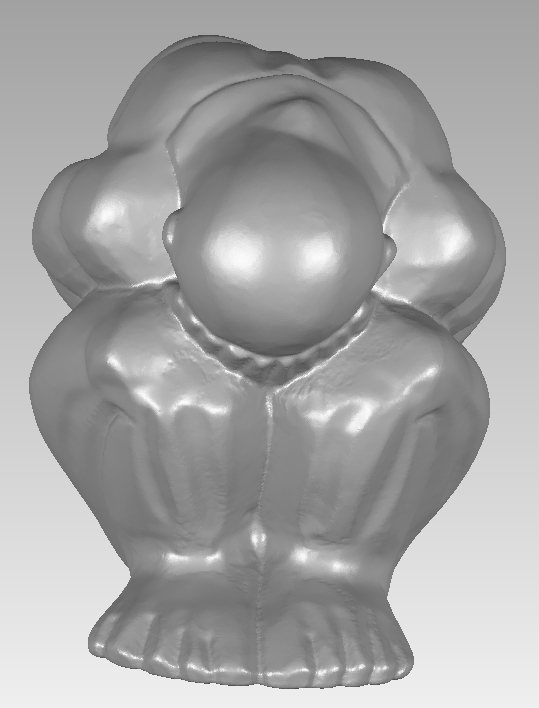
\includegraphics[width=\textwidth]{images/Mann_Front}
		\end{subfigure}
		\begin{subfigure}{0.4\textwidth}
			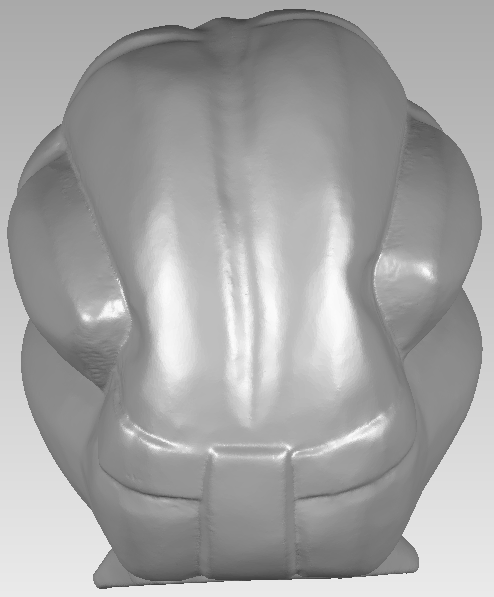
\includegraphics[width=\textwidth]{images/Mann_Back}
		\end{subfigure}
	\end{figure}
\end{frame}

\begin{frame}{Mann-Modell: 123D Catch}
	\begin{figure}
		\begin{subfigure}{0.4\textwidth}
			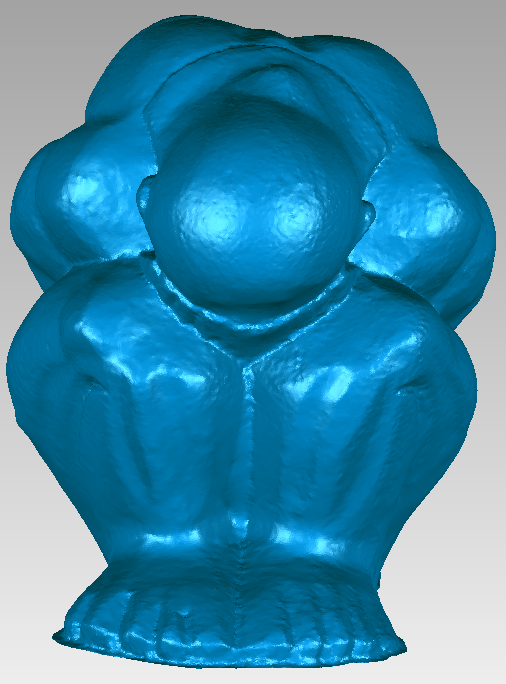
\includegraphics[width=\textwidth]{images/Mann_SFM_Front}
		\end{subfigure}
		\begin{subfigure}{0.4\textwidth}
			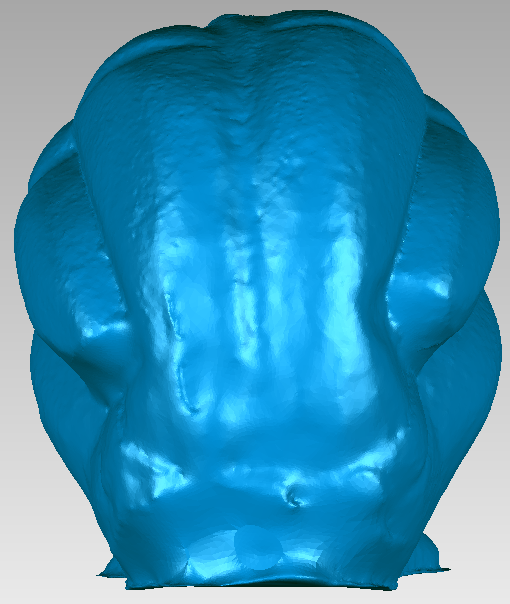
\includegraphics[width=\textwidth]{images/Mann_SFM_Back}
		\end{subfigure}
	\end{figure}
\end{frame}

\begin{frame}{Mann-Modell: Evaluierung}

	\begin{itemize}
	\item 3 Messungen
		\begin{itemize}
		\item Fußlänge
		\item Armlänge
		\item Hosenbund
		\end{itemize}
	\item $\varnothing$ Fehler Scan: $\pm 0,93$mm
	\item $\varnothing$ Fehler 123D Catch: $\pm 2,62$mm
	\item Volumen Scan: $544.250,14mm^3$
	\item Volumen 123D Catch: $583.912,27mm^3$
		\begin{itemize}
		\item Differenz: $39.662,13mm^3(7,28\%)$
		\end{itemize}
	\end{itemize}
	
\end{frame}

\begin{frame}{Objekte}
	\includegraphics[width=3.5cm]{images/Budha/Budha_Original.jpg}
	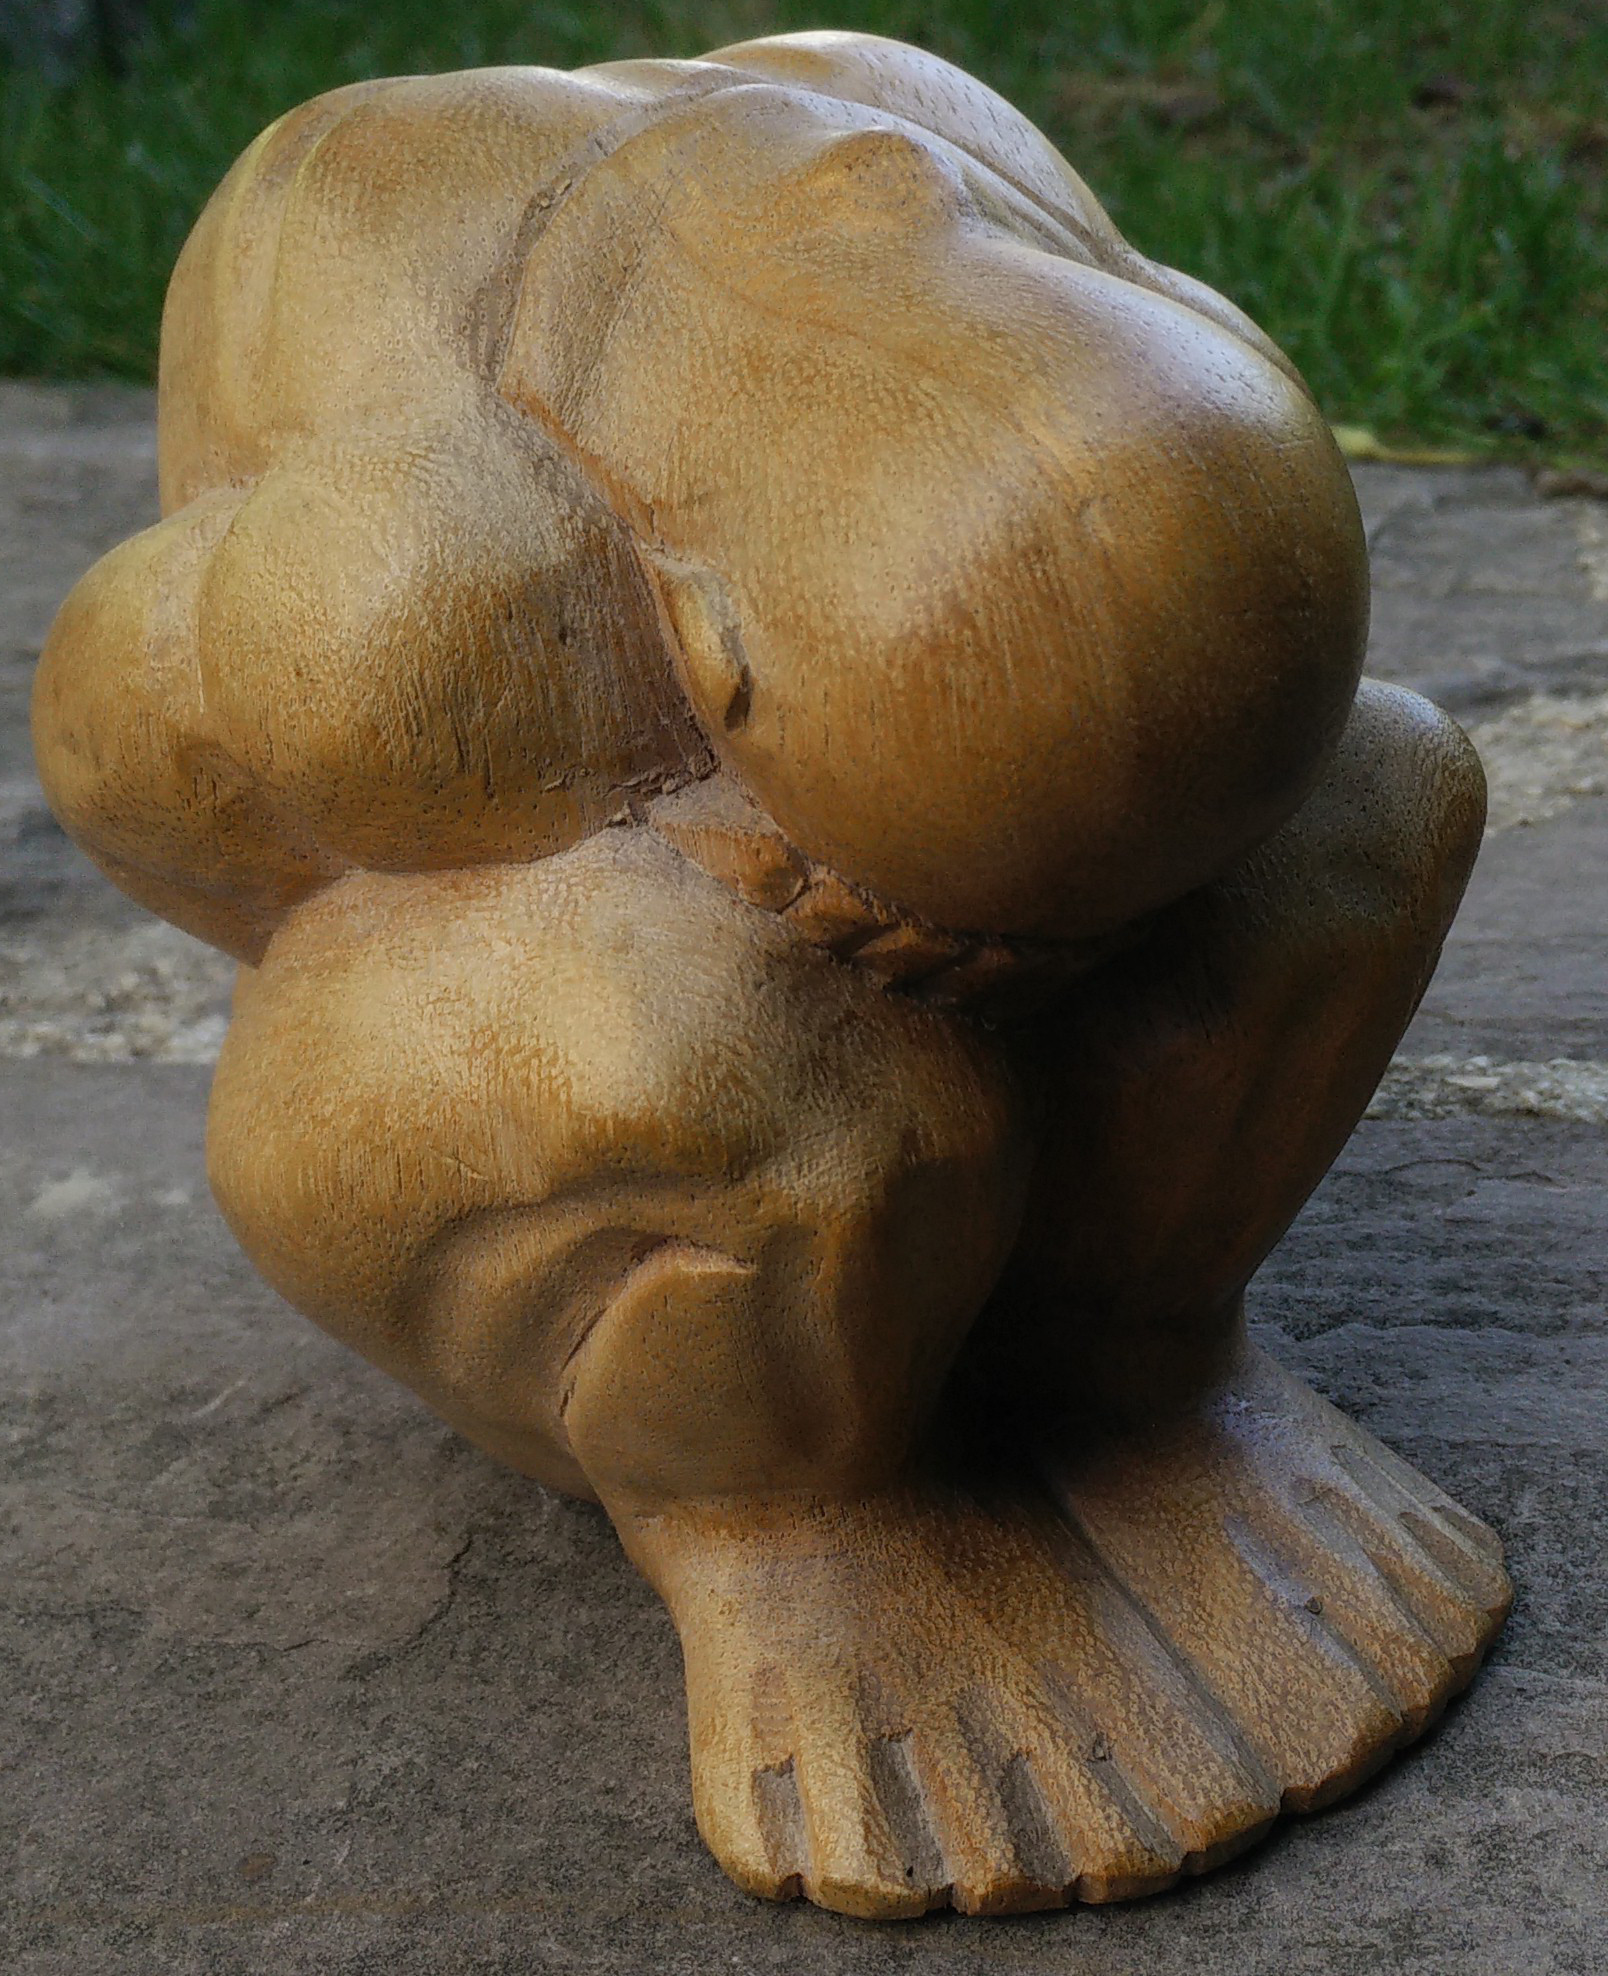
\includegraphics[width=3.5cm]{images/Mann_Original.jpg}
	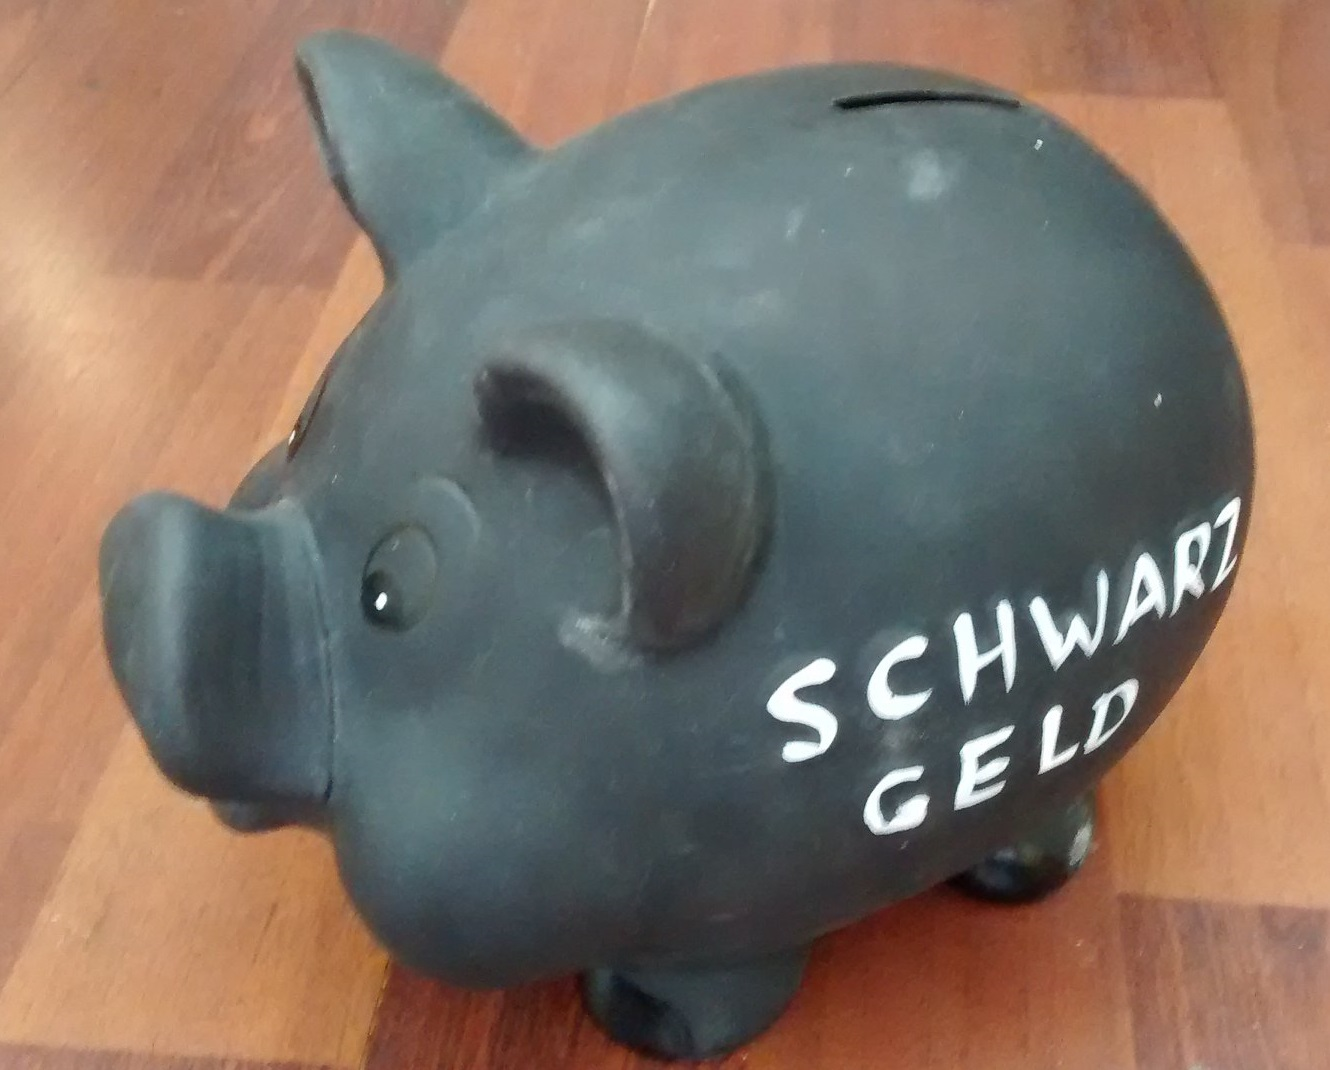
\includegraphics[width=5cm]{images/sparschwein/photo.jpg}
\end{frame}

\begin{frame}{Finale Modelle}
	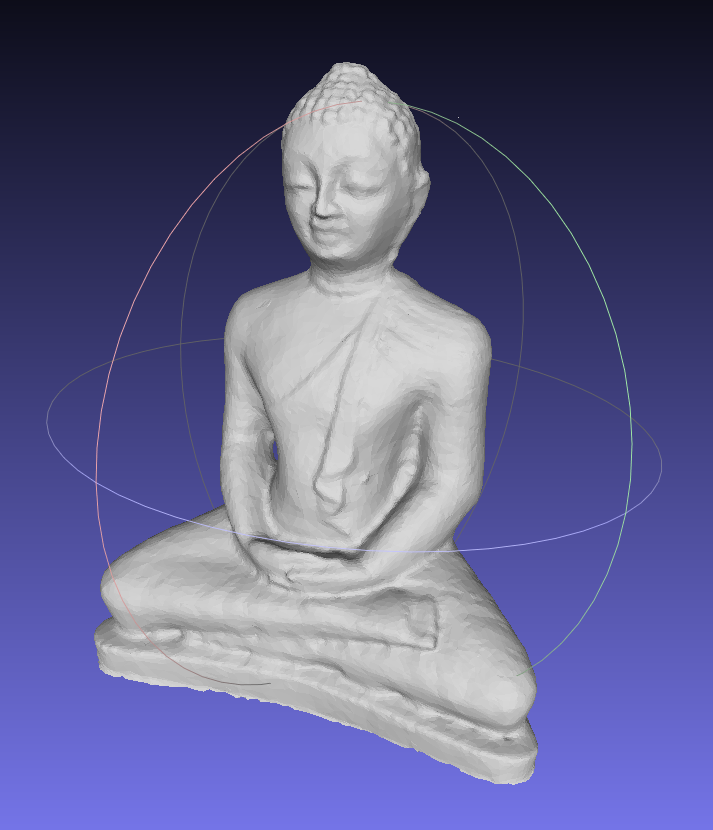
\includegraphics[width=3.5cm]{./Images/Budha/Budha_SfM_Untextured.png}
	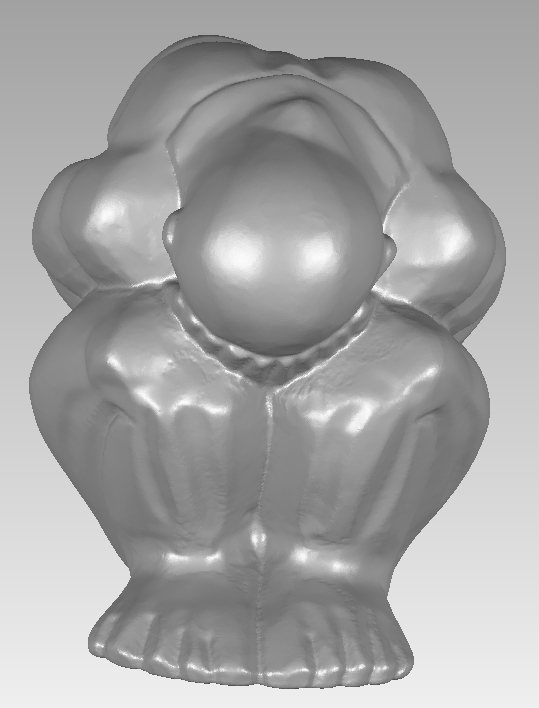
\includegraphics[width=3.5cm]{images/Mann_Front}
	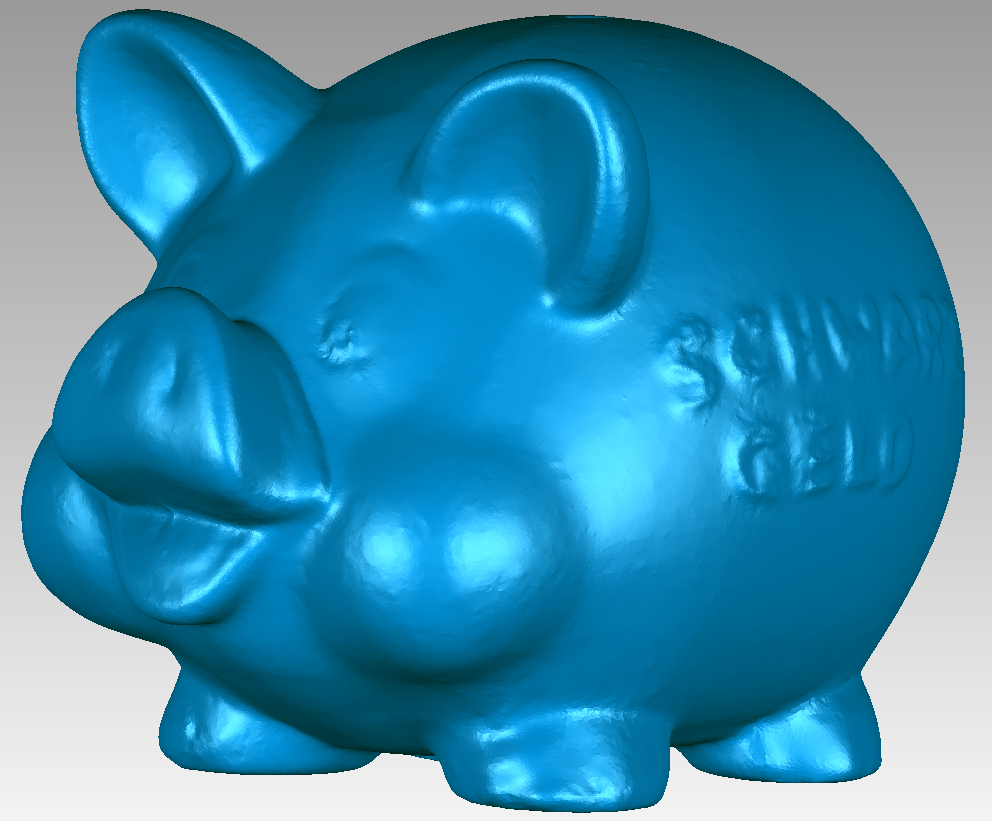
\includegraphics[width=4.5cm]{images/sparschwein/final}
\end{frame}
\end{document}